% -*- TeX-engine: xetex; eval: (auto-fill-mode 0); eval: (visual-line-mode 1); -*-
% Compile with XeLaTeX

%%%%%%%%%%%%%%%%%%%%%%%
% Option 1: Slides: (comment for handouts)   %
%%%%%%%%%%%%%%%%%%%%%%%

\documentclass[slidestop,compress,mathserif,11pt,t,professionalfonts,xcolor=table]{beamer}

% solution stuff
\newcommand{\solnMult}[1]{
\only<1>{#1}
\only<2->{\red{\textbf{#1}}}
}
\newcommand{\soln}[1]{\textit{#1}}

%%%%%%%%%%%%%%%%%%%%%%%%%%%%%%%
% Option 2: Handouts, without solutions (post before class)    %
%%%%%%%%%%%%%%%%%%%%%%%%%%%%%%%

% \documentclass[11pt,containsverbatim,handout,xcolor=xelatex,dvipsnames,table]{beamer}

% % handout layout
% \usepackage{pgfpages}
% \pgfpagesuselayout{4 on 1}[letterpaper,landscape,border shrink=5mm]

% % solution stuff
% \newcommand{\solnMult}[1]{#1}
% \newcommand{\soln}[1]{}

%%%%%%%%%%%%%%%%%%%%%%%%%%%%%%%%%%%%
% Option 3: Handouts, with solutions (may post after class if need be)    %
%%%%%%%%%%%%%%%%%%%%%%%%%%%%%%%%%%%%

% \documentclass[11pt,containsverbatim,handout,xcolor=xelatex,dvipsnames,table]{beamer}

% % handout layout
% \usepackage{pgfpages}
% \pgfpagesuselayout{4 on 1}[letterpaper,landscape,border shrink=5mm]

% % solution stuff
% \newcommand{\solnMult}[1]{\red{\textbf{#1}}}
% \newcommand{\soln}[1]{\textit{#1}}

%%%%%%%%%%
% Load style file, defaults  %
%%%%%%%%%%

%%%%%%%%%%%%%%%%
% Themes
%%%%%%%%%%%%%%%%

% See http://deic.uab.es/~iblanes/beamer_gallery/ for mor options

% Style theme
\usetheme{metropolis}

% Color theme
%\usecolortheme{seahorse}

% Helvetica Neue Light for most text
%\usepackage{fontspec}
%\setsansfont{Helvetica Neue Light}

%%%%%%%%%%%%%%%%
% Packages
%%%%%%%%%%%%%%%%

\usepackage{geometry}
\usepackage{graphicx}
\usepackage{amssymb}
\usepackage{epstopdf}
\usepackage{amsmath}  	% this permits text in eqnarray among other benefits
\usepackage{url}		% produces hyperlinks
\usepackage[english]{babel}
\usepackage{colortbl}	% allows for color usage in tables
\usepackage{multirow}	% allows for rows that span multiple rows in tables
\usepackage{color}		% this package has a variety of color options
\usepackage{pgf}
\usepackage{calc}
\usepackage{ulem}
\usepackage{multicol}
\usepackage{textcomp}
\usepackage{listings}
\usepackage{changepage}
\usepackage{tikz}
\usetikzlibrary{trees}		% for probability trees
\usepackage{fancyvrb}	% for colored code chunks
\usepackage{nameref}

%%%%%%%%%%%%%%%%
% Remove navigation symbols
%%%%%%%%%%%%%%%%

\beamertemplatenavigationsymbolsempty
\hypersetup{pdfpagemode=UseNone} % don't show bookmarks on initial view

%%%%%%%%%%%%%%%%
% User defined colors
%%%%%%%%%%%%%%%%

% Pantone 2016 Spring colors
% https://atelierbram.github.io/c-tiles16/colorscheming/pantone-spring-2016-colortable.html
% update each semester or year

\xdefinecolor{custom_blue}{rgb}{0.01, 0.31, 0.52} % Snorkel Blue
\xdefinecolor{custom_darkBlue}{rgb}{0.20, 0.20, 0.39} % Reflecting Pond  
\xdefinecolor{custom_orange}{rgb}{0.96, 0.57, 0.42} % Cadmium Orange
\xdefinecolor{custom_green}{rgb}{0, 0.47, 0.52} % Biscay Bay
\xdefinecolor{custom_red}{rgb}{0.58, 0.32, 0.32} % Marsala

\xdefinecolor{custom_lightGray}{rgb}{0.78, 0.80, 0.80} % Glacier Gray
\xdefinecolor{custom_darkGray}{rgb}{0.35, 0.39, 0.43} % Stormy Weather

%%%%%%%%%%%%%%%%
% Template colors
%%%%%%%%%%%%%%%%

%\setbeamercolor*{palette primary}{fg=white,bg= custom_blue}
%\setbeamercolor*{palette secondary}{fg=black,bg= custom_blue!80!black}
%\setbeamercolor*{palette tertiary}{fg=white,bg= custom_blue!80!black!80}
%\setbeamercolor*{palette quaternary}{fg=white,bg= custom_blue}
%
%\setbeamercolor{structure}{fg= custom_blue}
%\setbeamercolor{frametitle}{bg= custom_blue!90}
%\setbeamertemplate{blocks}[shadow=false]
%\setbeamersize{text margin left=2em,text margin right=2em}

%%%%%%%%%%%%%%%%
% Styling fonts, bullets, etc.
%%%%%%%%%%%%%%%%
%
%% title slide
%\setbeamerfont{title}{size=\large,series=\bfseries}
%\setbeamerfont{subtitle}{size=\large,series=\mdseries}
%%\setbeamerfont{institute}{size=\large,series=\mdseries}
%
% color of alerted text
\setbeamercolor{alerted text}{fg=custom_orange}

% styling of itemize bullets
\setbeamercolor{item}{fg=custom_blue}
\setbeamertemplate{itemize item}{{{\small$\blacktriangleright$}}}
\setbeamercolor{subitem}{fg=custom_blue}
\setbeamertemplate{itemize subitem}{{\textendash}}
\setbeamerfont{itemize/enumerate subbody}{size=\footnotesize}
\setbeamerfont{itemize/enumerate subitem}{size=\footnotesize}

% styling of enumerate bullets
\setbeamertemplate{enumerate item}{\insertenumlabel.}

%\setbeamerfont{enumerate item}{family={\fontspec{Helvetica Neue}}}
%\setbeamerfont{enumerate subitem}{family={\fontspec{Helvetica Neue}}}
%\setbeamerfont{enumerate subsubitem}{family={\fontspec{Helvetica Neue}}}

% make frame titles small to make room in the slide
\setbeamerfont{frametitle}{size=\small} 




%% set Helvetica Neue font for frame and section titles
%\setbeamerfont{frametitle}{family={\fontspec{Helvetica Neue}}}
%\setbeamerfont{sectiontitle}{family={\fontspec{Helvetica Neue}}}
%\setbeamerfont{section in toc}{family={\fontspec{Helvetica Neue}}}
%\setbeamerfont{subsection in toc}{family={\fontspec{Helvetica Neue}}, size=\small}
%\setbeamerfont{footline}{family={\fontspec{Helvetica Neue}}}
%\setbeamerfont{subsection in toc}{family={\fontspec{Helvetica Neue}}}
%\setbeamerfont{block title}{family={\fontspec{Helvetica Neue}}}
%
%%%%%%%%%%%%%%%%%
%% New fonts accessed by fontspec package
%%%%%%%%%%%%%%%%%
%
%% Monaco font for code
%\newfontfamily{\monaco}{Monaco}

%%%%%%%%%%%%%%%%
% Color text commands
%%%%%%%%%%%%%%%%

%orange
\newcommand{\orange}[1]{\textit{\textcolor{custom_orange}{#1}}}

% yellow
\newcommand{\yellow}[1]{\textit{\textcolor{yellow}{#1}}}

% blue
\newcommand{\blue}[1]{\textit{\textcolor{blue}{#1}}}

% green
\newcommand{\green}[1]{\textit{\textcolor{custom_green}{#1}}}

% red
\newcommand{\red}[1]{\textit{\textcolor{custom_red}{#1}}}

% dark gray
\newcommand{\darkgray}[1]{\textit{\textcolor{custom_darkGray}{#1}}}

% light gray
\newcommand{\lightgray}[1]{\textit{\textcolor{custom_lightGray}{#1}}}

% pink
\newcommand{\pink}[1]{\textit{\textcolor{pink}{#1}}}


%%%%%%%%%%%%%%%%
% Custom commands
%%%%%%%%%%%%%%%%

% empty box for probability tree frame
\newcommand{\emptybox}[2]{
	\fbox{ \begin{minipage}{#1} \hfill\vspace{#2} \end{minipage} }
}

% cancel
\newcommand{\cancel}[1]{%
    \tikz[baseline=(tocancel.base)]{
        \node[inner sep=0pt,outer sep=0pt] (tocancel) {#1};
        \draw[red, line width=0.5mm] (tocancel.south west) -- (tocancel.north east);
    }%
}

% degree
\newcommand{\degree}{\ensuremath{^\circ}}

% cite
\newcommand{\ct}[1]{
\vfill
{\tiny #1}}

% Note
\newcommand{\Note}[1]{
\rule{2.5cm}{0.25pt} \\ \textit{\footnotesize{\textcolor{custom_red}{Note:} \textcolor{custom_darkGray}{#1}}}}

% Remember
\newcommand{\Remember}[1]{\textit{\scriptsize{\textcolor{custom_red}{Remember:} #1}}}

% links: webURL, webLink
\newcommand{\webURL}[1]{\urlstyle{same}{\textit{\textcolor{custom_blue}{\url{#1}}}}}
\newcommand{\webLink}[2]{\href{#1}{\textcolor{custom_blue}{{#2}}}}

% mail
\newcommand{\mail}[1]{\href{mailto:#1}{\textit{\textcolor{custom_blue}{#1}}}}

% highlighting: hl, hlGr, mathhl
\newcommand{\hl}[1]{\textit{\textcolor{custom_blue}{#1}}}
\newcommand{\hlGr}[1]{\textit{\textcolor{custom_green}{#1}}}
\newcommand{\mathhl}[1]{\textcolor{custom_blue}{\ensuremath{#1}}}

% example
\newcommand{\ex}[1]{\textcolor{blue}{{{\small (#1)}}}}

% twocol: two columns
\newenvironment{twocol}[4]{
\begin{columns}[c]
\column{#1\textwidth}
#3
\column{#2\textwidth}
#4
\end{columns}
}

% threecol: three columns
\newenvironment{threecol}[6]{
\begin{columns}[c]
\column{#1\textwidth}
#4
\column{#2\textwidth}
#5
\column{#3\textwidth}
#6
\end{columns}
}

% slot (for probability calculations)
\newenvironment{slot}[2]{
\begin{array}{c} 
\underline{#1} \\ 
#2
\end{array}
}

% pr: left and right parentheses
\newcommand{\pr}[1]{
\left( #1 \right)
}

%%%%%%%%%%%%%%%%
% Custom blocks
%%%%%%%%%%%%%%%%

% activity: less commonly used
\newcommand{\activity}[2]{
\setbeamertemplate{itemize item}{{{\small\textcolor{custom_orange}{$\blacktriangleright$}}}}
\setbeamercolor{block title}{fg=white, bg=custom_orange}
\setbeamerfont{block title}{size=\small}
\setbeamercolor{block body}{fg=black, bg=custom_orange!20!white!80}
\setbeamerfont{block body}{size=\small}
\begin{block}{Activity: #1}
\setlength\abovedisplayskip{0pt}
#2
\end{block}
}

% app: application exercise
\newcommand{\app}[2]{
\setbeamercolor{block title}{fg=white,bg=custom_green}
\setbeamercolor{block body}{fg=black,bg=custom_green!20!white!80}
\begin{block}{{\small Application exercise: #1}}
#2
\end{block}
}

% disc: discussion question
\newcommand{\disc}[1]{
\vspace*{-2ex}
\setbeamercolor{block body}{bg=custom_blue!25!white!80, fg=custom_blue!55!black!95}
\begin{block}{\vspace*{-3ex}}
#1
\end{block}
\vspace*{-1ex}
}

% clicker: clicker question
\newcommand{\clicker}[1]{
\setbeamercolor{block title}{bg=custom_blue!80!white!50,fg=custom_blue!30!black!90}
\setbeamercolor{block body}{bg=custom_blue!20!white!80,fg=custom_blue!30!black!90}
\begin{block}{\vspace*{-0.2ex}{\footnotesize Your turn}\vspace*{-0.2ex}}
#1
\end{block}
}

% formula
\newcommand{\formula}[2]{
\setbeamercolor{block title}{bg=custom_blue!40!white!60,fg=custom_blue!55!black!95}
\begin{block}{{\small#1}}
#2
\end{block}
}

% code
\newcommand{\Rcode}[1]{
{\monaco {\footnotesize \textcolor{custom_darkBlue}{#1}}}
}

% output
\newcommand{\Rout}[1]{
{\monaco {\footnotesize \textcolor{custom_darkGray}{#1}}}
}

%%%%%%%%%%%%%%%%
% Change margin
%%%%%%%%%%%%%%%%

\newenvironment{changemargin}[2]{%
\begin{list}{}{%
\setlength{\topsep}{0pt}%
\setlength{\leftmargin}{#1}%
\setlength{\rightmargin}{#2}%
\setlength{\listparindent}{\parindent}%
\setlength{\itemindent}{\parindent}%
\setlength{\parsep}{\parskip}%
}%
\item}{\end{list}}

%%%%%%%%%%%%%%%%
% Footnote
%%%%%%%%%%%%%%%%

\long\def\symbolfootnote[#1]#2{\begingroup%
\def\thefootnote{\fnsymbol{footnote}}\footnote[#1]{#2}\endgroup}

%%%%%%%%%%%%%%%%
% Graphics
%%%%%%%%%%%%%%%%

\DeclareGraphicsRule{.tif}{png}{.png}{`convert #1 `dirname #1`/`basename #1 .tif`.png}

%%%%%%%%%%%%%%%%
% Slide number
%%%%%%%%%%%%%%%%

\setbeamertemplate{footline}{%
    \raisebox{5pt}{\makebox[\paperwidth]{\hfill\makebox[20pt]{\color{gray}
          \scriptsize\insertframenumber}}}\hspace*{5pt}}

          
%%%%%%%%%%%%%%%%
% Remove page numbers
%%%%%%%%%%%%%%%%

\newcommand{\removepagenumbers}{% 
  \setbeamertemplate{footline}{}
}

%%%%%%%%%%%%%%%%
% TOC slides
%%%%%%%%%%%%%%%%

\setbeamertemplate{section in toc}{\inserttocsectionnumber.~\inserttocsection}
\setbeamertemplate{subsection in toc}{$\qquad$\inserttocsubsectionnumber.~\inserttocsubsection \\}

\AtBeginSection[] 
{ 
  \addtocounter{framenumber}{-1} 
  % 
  {\removepagenumbers 
  {\small
    \begin{frame}<beamer> 
    \frametitle{Outline} 
    \tableofcontents[currentsection] 
  \end{frame} 
  } 
  }
} 

\AtBeginSubsection[] 
{ 
  \addtocounter{framenumber}{-1} 
  % 
  {\removepagenumbers 
  {\small
    \begin{frame}<beamer> 
    \frametitle{Outline} 
    \tableofcontents[currentsection,currentsubsection] 
  \end{frame} 
  } 
  }
}
% Course Name
\newcommand{\CourseName}{LBJ - SDA - Spring 2024}
\newcommand{\InstituteName}{University of Texas}

% Personal Info
\newcommand{\FirstName}{Sergio}
\newcommand{\LastName}{Garcia-Rios}

% Electronic Info
\newcommand{\PersonalSite}{https://garciarios.github.io}
\newcommand{\CourseSite}{http://garciarios.github.io/govt_3990/}
\newcommand{\Email}{garcia.rios@cornell.edu}

% Exam Dates
\newcommand{\ExamADate}{Feb 24, Wed}
\newcommand{\ExamBDate}{Mar 30, Wed}
\newcommand{\FinalDate}{May 5, Thu - 7-10pm}
% ALT ALT
% % Course Name
\newcommand{\CourseName}{Sta 101 - Spring 2016}
\newcommand{\InstituteName}{Duke University, Department of Statistical Science}

% Personal Info
\newcommand{\FirstName}{Anthea}
\newcommand{\LastName}{Monod}

% Electronic Info
\newcommand{\PersonalSite}{https://stat.duke.edu/people/anthea-monod.html}
\newcommand{\CourseSite}{https://stat.duke.edu/courses/Spring16/sta101.002}
\newcommand{\Email}{anthea@stat.duke.edu}

% Exam Dates
\newcommand{\ExamADate}{Feb 25, Thu}
\newcommand{\ExamBDate}{Mar 31, Thu}
\newcommand{\FinalDate}{???}

%%%%%%%%%%%
% Cover slide info    %
%%%%%%%%%%%

\title{Unit 2: Probability and distributions}
\subtitle{1. Probability and conditional probability}
\author{\CourseName}
\date{}
\institute{\InstituteName}


%%%%%%%%%%%%%%%%%%%%%%%%%
% Begin document and set Helvetica Neue font   %
%%%%%%%%%%%%%%%%%%%%%%%%%

\begin{document}
%\fontspec[Ligatures=TeX]{Helvetica Neue Light}

%%%%%%%%%%%%%%%%%%%%%%%%%%%%%%%%%%%

% Title Page

\begin{frame}[plain]

\titlepage

\vfill

{\scriptsize \webLink{\PersonalSite}{Dr. \LastName{}} \hfill Slides posted at  \webURL{\CourseSite}}

\addtocounter{framenumber}{-1} 

\end{frame}


%\section{Readiness assessment}

%%%%%%%%%%%%%%%%%%%%%%%%%%%%%%%%%%%%

%\begin{frame}
%\frametitle{Readiness assessment}
%
%\begin{itemize}
%
%\item 15 minutes individual -- turn your clicker over when you're done
%
%\item 10 minutes team -- put your team name on the front of the scratch 
%off sheet + Lab time + note if anyone from your team is missing
%
%\end{itemize}
%
%\end{frame}
%
%%%%%%%%%%%%%%%%%%%%%%%%%%%%%%%%%%%%

\section{Main ideas}

%%%%%%%%%%%%%%%%%%%%%%%%%%%%%%%%%%%%

\subsection{Disjoint and independent do not mean the same thing}
\label{mi1}

%%%%%%%%%%%%%%%%%%%%%%%%%%%%%%%%%%%%

\begin{frame}
\frametitle{1. Disjoint and independent do not mean the same thing}

\begin{itemize}

\item \hl{Disjoint (mutually exclusive) events} cannot happen at the same time
\begin{itemize} \pause
\item A voter cannot register as a Democrat and a Republican at the same time
\item But they might be a Republican and a Moderate at the same time -- 
\hl{non-disjoint events}
\item For disjoint A and B: $P(A~and~B) = 0$
\end{itemize}

\pause

\item If A and B are \hl{independent events}, having information on A does 
not tell us anything about B (and vice versa)
\begin{itemize}
\item If A and B are independent: 
\begin{itemize}
\item $P(A~|~B) = P(A)$
\item $P(A~and~B) = P(A) \times P(B)$
\end{itemize}
\end{itemize}

\end{itemize}
\end{frame}

%%%%%%%%%%%%%%%%%%%%%%%%%%%%%%%%%%%%

\subsection{Application of the addition rule depends on disjointness of events}
\label{mi2}

%%%%%%%%%%%%%%%%%%%%%%%%%%%%%%%%%%%%

\begin{frame}
\frametitle{2. Application of the addition rule depends on disjointness of events}

\begin{itemize}

\item \hl{General addition rule:} P(A or B) = P(A) + P(B) - P(A and B)

\item A or B = either A or B or both

\end{itemize}

\vspace{0.5cm}

\pause

\twocol{0.5}{0.5}{
\textbf{disjoint events:} \\
P(A or B) \\
= P(A) + P(B) - P(A and B) \\
\only<3->{= 0.4 + 0.3 - 0 = 0.7} 
\begin{center}
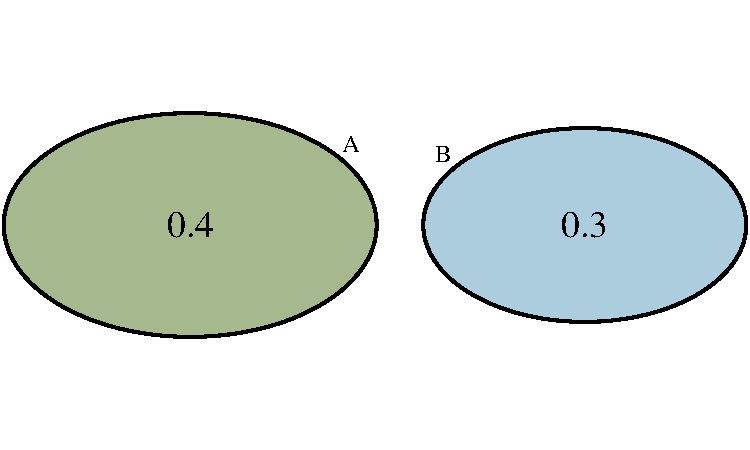
\includegraphics[width = 0.9\textwidth]{figures/venn/venn_disjoint.pdf} 
\end{center} \pause
}
{

\textbf{non-disjoint events:} \\
P(A or B) \\
= P(A) + P(B) - P(A and B) \\ 
\only<5->{ = 0.4 + 0.3 - 0.02 = 0.68}

\begin{center}
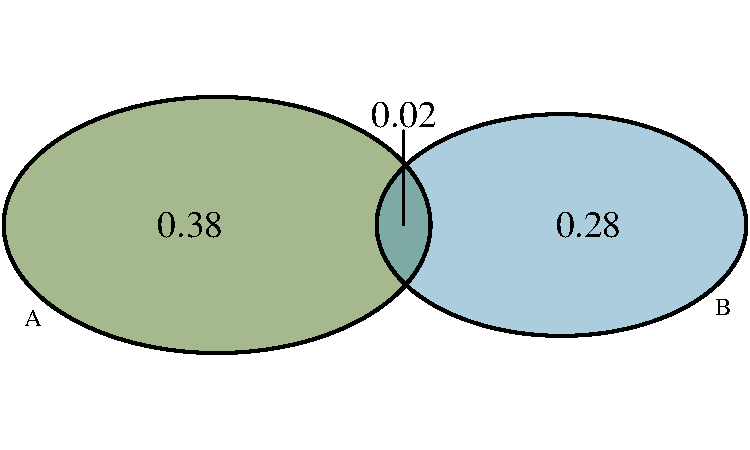
\includegraphics[width = 0.9\textwidth]{figures/venn/venn_non_disjoint.pdf}
\end{center}
}

\end{frame}

%%%%%%%%%%%%%%%%%%%%%%%%%%%%%%%%%%%%
%
%\subsection{Bayes' theorem works for all types of events}
%\label{mi3}
%
%%%%%%%%%%%%%%%%%%%%%%%%%%%%%%%%%%%%%
%
%\begin{frame}
%\frametitle{3. Bayes' theorem works for all types of events}
%
%\begin{itemize}
%
%\item \hl{Bayes' theorem:} $P(A~|~B) = \frac{P(A~and~B)(}{P(B)}$
%
%\pause
%
%\item ... can be rewritten as: $P(A~and~B) = P(A~|~B) \times P(B)$
%
%\end{itemize}
%
%\pause
%
%\vspace{0.5cm}
%
%\twocol{0.5}{0.5}{
%\textbf{disjoint events:}
%
%\begin{itemize}
%\item We know P(A $|$ B) = 0, since if B happened A could not have happened
%\pause
%\item P(A and B) \\
%= P(A $|$ B) $\times$ P(B) \\
%\pause
%= \red{0} $\times$ P(B) = 0
%\end{itemize}
%}
%{
%\pause
%
%\textbf{independent events:}
%
%\begin{itemize}
%\item We know P(A $|$ B) = P(A), since knowing B doesn't tell us anything about A
%\pause
%\item P(A and B) \\
%= P(A $|$ B) $\times$ P(B) \\
%\pause
%= \red{P(A)} $\times$ P(B)
%\end{itemize}
%}
%
%\end{frame}

%%%%%%%%%%%%%%%%%%%%%%%%%%%%%%%%%%%%

\begin{frame}
\frametitle{}

\vfill

\app{2.1 Probability and conditional probability}{}

\vfill

\end{frame}



\subsection{Probability trees are useful for conditional probability calculations}
\label{mi1}

%%%%%%%%%%%%%%%%%%%%%%%%%%%%%%%%%%%

\begin{frame}
\frametitle{1. Probability trees are useful for conditional probability calculations}

\begin{itemize}

\item Probability trees are useful for organizing information in conditional probability calculations

\item They're especially useful in cases where you know P(A $|$ B), along with some other information, and you're asked for P(B $|$ A)

\end{itemize}

\end{frame}

%%%%%%%%%%%%%%%%%%%%%%%%%%%%%%%%%%%

\subsection{Bayesian inference: start with a prior, collect data, calculate posterior, make a decision or iterate}
\label{mi2}

%%%%%%%%%%%%%%%%%%%%%%%%%%%%%%%%%%%%

\begin{frame}
\frametitle{2. Bayesian inference: start with a prior, collect data, calculate posterior, make a decision or iterate}

\begin{itemize}[<+->]

\item In Bayesian inference, probabilities are at times interpreted as \textbf{degrees of belief}.

\item You start with a set of \textbf{prior beliefs} (or prior probabilities).

\item You observe some data.

\item Based on that data, you update your beliefs.  

\item These new beliefs are called \textbf{posterior beliefs} (or posterior probabilities), because they are \textbf{post}-data.

\item You can iterate this process.

\end{itemize}

\end{frame}

%%%%%%%%%%%%%%%%%%%%%%%%%%%%%%%%%%%%

\begin{frame}
\frametitle{Dice game}

We'll play a game to demonstrate this approach:

\begin{itemize}

\item Two dice: 6-sided and 12-sided
\begin{itemize}
\item I keep one die on my cellphone and one die on my computer
\end{itemize}

\pause

\item The ``good die'' is the 12-sided die.

\pause

\item Ultimate goal: come to a class consensus about whether the die on the cellphone or the die on the computer is the ``good die''

\pause

\item We will start with priors, collect data, and calculate posteriors, and make a decision or iterate until we're ready to make a decision

\end{itemize}

\end{frame}

%%%%%%%%%%%%%%%%%%%%%%%%%%%%%%%%%%%%

\begin{frame}
\frametitle{Prior probabilities}

\begin{itemize}

\item At each roll I tell you whether you won or not (win = $\ge 4$)
\begin{itemize}
\item P(win $\mid$ 6-sided die) = 0.5 $\rightarrow$ bad die
\item P(win $\mid$ 12-sided die) = 0.75 $\rightarrow$ good die
\end{itemize}

\pause

\item The two competing claims are
\begin{itemize}
\item[] $H_1$: Good die is on the cellphone 
\item[] $H_2$: Good die is on the computer
\end{itemize}

\pause

\item Since initially you have no idea which is true, you can assign equal \hl{prior probabilities} to the hypotheses
\begin{itemize}
\item[] P($H_1$ is true) = 0.5 
\item[] P($H_2$ is true) = 0.5 
\end{itemize}

\end{itemize}

\end{frame}

%%%%%%%%%%%%%%%%%%%%%%%%%%%%%%%%%%%%

\begin{frame}
\frametitle{Rules of the game}

\begin{itemize}

\item You won't know which die I'm holding in which hand, left (Computer) or right (Cellphone). {\footnotesize left = YOUR left}

\item You pick die (L or R), I roll it, and I tell you if you win or not, where winning is getting a number $\ge$ 4. If you win, you get a piece of candy. If you lose, I get to keep the candy.

\item We'll play this multiple times with different contestants.

\item I will not swap the sides the dice are on at any point.

\item You get to pick how long you want play, but there are costs associated with playing longer.

\end{itemize}

\end{frame}

%%%%%%%%%%%%%%%%%%%%%%%%%%%%%%%%%%%%

\begin{frame}
\frametitle{Hypotheses and decisions}

\begin{center}
\renewcommand\arraystretch{1.25}
\begin{tabular}{l | c | c | }
  			&\multicolumn{2}{c|}{\hl{Truth}} \\
\cline{2-3}
\hl{Decision}		& {\small L good, R bad}		& {L bad, R good} \\
\hline
Pick L		& \hlGr{You get candy!}			& \red{You lose all the candy :(} \\
\hline
Pick R		& \red{You lose all the candy :(}	& \hlGr{You get candy!} \\
\hline
\end{tabular}
\end{center}

\vspace{0.75cm}

\hl{Sampling isn't free!} \\
At each trial you risk losing pieces of candy if you lose (the die comes up $<$ 4). Too many trials means you won't have much candy left. And if we spend too much class time and we may not get through all the material.
	
\end{frame}

%%%%%%%%%%%%%%%%%%%%%%%%%%%%%%%%%%%%

\begin{frame}
\frametitle{Data and decision making}

\begin{center}
\renewcommand\arraystretch{1.25}
\begin{tabular}{l | c | c}
		& Choice (L or R)	& Result (win or loss) \\
\hline
Roll 1	& 				& 				\\
\hline
Roll 2	& 				& 				\\
\hline
Roll 3	& 				& 				\\
\hline
Roll 4	& 				& 				\\
\hline
Roll 5	& 				& 				\\
\hline
Roll 6	& 				& 				\\
\hline
Roll 7	& 				& 				\\
\hline
...		& 				& 				\\
\end{tabular}
\end{center}

\disc{What is your decision? How did you make this decision?}

\end{frame}

%%%%%%%%%%%%%%%%%%%%%%%%%%%%%%%%%%%%
%
%\begin{frame}
%\frametitle{Posterior probability}
%
%\begin{itemize}
%
%\item \hl{Posterior probability} is the probability of the hypothesis given the observed data: P(hypothesis $|$ data)
%
%\pause
%
%\item Using Bayes' theorem
%\begin{eqnarray*}
%P(hypothesis \mid data) &=& \frac{P(hypothesis~and~data)}{P(data)} \\
%\pause
%&=& \frac{P(data~|~hypothesis) \times P(hypothesis)}{P(data)}
%\end{eqnarray*}
%
%\end{itemize}
%
%\end{frame}

%%%%%%%%%%%%%%%%%%%%%%%%%%%%%%%%%%%%
%
%\begin{frame}
%\frametitle{}
%
%
%\disc{Calculate the posterior probability for the hypothesis chosen in the first roll, and discuss how this might influence your decision for the next roll.}
%% ALT ALT
%% \disc{Calculate the posterior probability after flipping the coin once.}
%
%% Set the overall layout of the tree
%\tikzstyle{level 1}=[level distance=3.5cm, sibling distance=3.5cm]
%\tikzstyle{level 2}=[level distance=3.5cm, sibling distance=1.5cm]
%
%% Define styles for bags
%\tikzstyle{bag} = [text width=4em, text centered]
%\tikzstyle{end} = [minimum width=3pt, inner sep=0pt]
%
%% Draw picture
%\hspace{-1.5cm}
%\begin{tikzpicture}[grow=right]
%\node[bag] {}
%    child {
%        node[bag] {\emptybox{0.5cm}{0.25cm}      }  
%            child {
%                node[end, label=right:
%                    {\emptybox{0.5cm}{0.25cm}      }] {}
%                edge from parent
%            }
%            child {
%                node[end, label=right:
%                    {\emptybox{0.5cm}{0.25cm}      }] {}
%                edge from parent
%            }
%            edge from parent
%    }
%    child {
%        node[bag] {\emptybox{0.5cm}{0.25cm}      }        
%            child {
%                node[end, label=right:
%                    {\emptybox{0.5cm}{0.25cm}      }] {}
%                edge from parent
%            }
%            child {
%                node[end, label=right:
%                    {\emptybox{0.5cm}{0.25cm}      }] {}
%                edge from parent
%            }
%            edge from parent
%    };
%\end{tikzpicture}
%
%\end{frame}


\begin{frame}{Bayesian probability and updating our priors}
\disc{Most companies drug test their employees before they start employment, and sometimes regularly during their employment as well. Suppose that a drug test for an illegal drugs is 97\% accurate in the case of a user of that drug, and 92\% accurate in the case of a non-user for that drug. Suppose also that 5\% of the entire population uses that drug.}\pause
\begin{itemize}


\item You are the hiring manager at a company that drug tests their employees. You have recently decided to hire a new employee. What is the prior probability that this employee is a user of this drug? (You may assume that this prospective employee is a randomly drawn person from the population.)\pause

	\begin{itemize} 
	\item \red{P(drug user) = 0.05}
	\end{itemize}
\end{itemize}
\end{frame}


\begin{frame}
\begin{itemize}
\item The prospective employee gets drug tested, and the test comes out to be positive. What is the probability that they are actually a user for the drug? What is this probability called? Sketch a probability tree for this question. \pause

	\begin{itemize}
	\item \red{P(drug user $|$ +) $\rightarrow$ posterior probability} \pause
	\end{itemize}
\end{itemize}

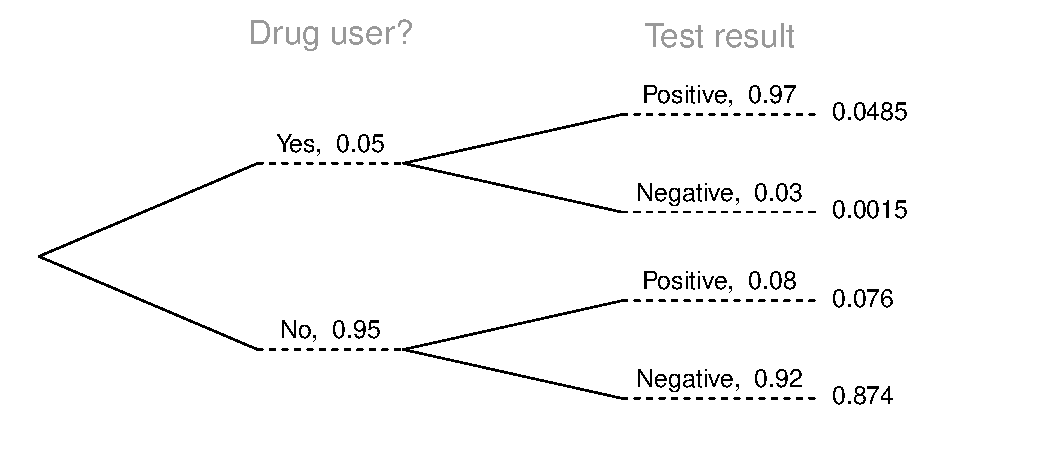
\includegraphics[width = \textwidth]{figures/test1.pdf}

\end{frame}


\end{document}

\begin{frame}
\begin{itemize}

\item When the employee finds out that they tested positive, they refuse the test results, and say they would like to be tested again. What is the new prior probability you should use for this employee being a user of this drug? \pause

\begin{itemize}
\item \red{P(drug user) = 0.39} \pause
\end{itemize}

\item The employee tests positive again in the second test. Should the new probability of them actually being a user of this drug be higher or lower than what you calculated before, or the same? Answer this question before you actually complete the calculations. \pause
\begin{itemize}
\item \red{Higher.}
\end{itemize}
\end{itemize}
\end{frame}

\begin{frame}
\begin{itemize}
\item Finally, calculate the new updated probability that this employee is a user of this drug. When answering this question sketch a probability tree, take a picture, and upload to Sakai as an attachment.
\begin{itemize}

\item \red{P(drug user $|$ +) $\rightarrow$ posterior probability} \pause

\end{itemize}
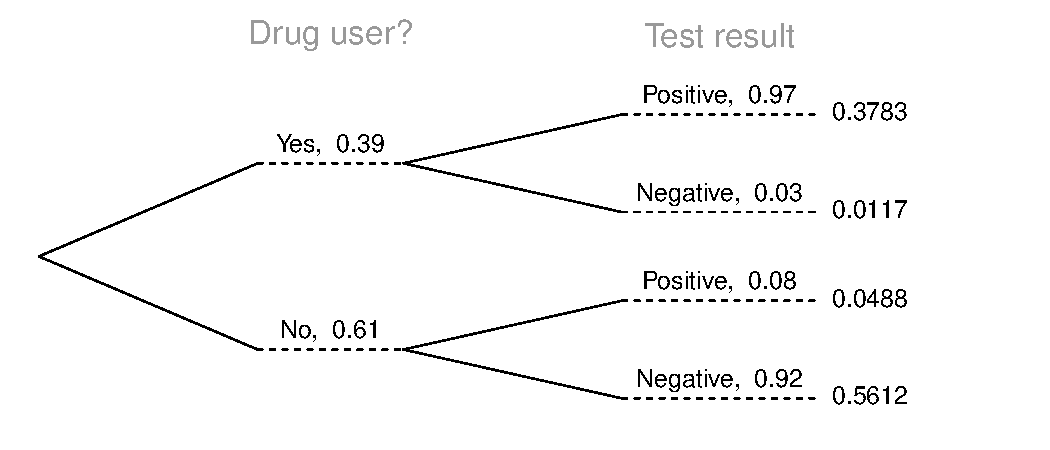
\includegraphics[width = \textwidth]{figures/test2.pdf} \pause

\item Based on these results, would you hire this employee? Why or why not?

\begin{itemize}
\item\red{No, quite likely that the employee is a drug user.}
\end{itemize}
\end{itemize}

\end{frame}



%%%%%%%%%%%%%%%%%%%%%%%%%%%%%%%%%%%%

\subsection{Posterior probability and p-value do not mean the same thing}
\label{mi3}

%%%%%%%%%%%%%%%%%%%%%%%%%%%%%%%%%%%%

\begin{frame}
\frametitle{3. Posterior probability and p-value do not mean the same thing}

\begin{itemize}

\item $\hl{p-value}:$ P(observed or more extreme outcome $|$ null hypothesis is true)
\begin{itemize}
\item This is more like P(data $|$ hyp) than P(hyp $|$ data).
\end{itemize}

\item $\hl{posterior}:$ P(hypothesis $|$ data)

\item Bayesian approach avoids the counter-intuitive Frequentist p-value for decision making, and more advanced Bayesian techniques offer flexibility not present in Frequentist models

\item \hl{Watch out!} \\
\begin{itemize}
\item $\hl{Bayes}$: A good prior helps, a bad prior hurts, but the prior matters less the more data you have.
\item $\hl{p-value}$: {It is really easy to mess up p-values}: \webLink{https://sakai.duke.edu/access/content/group/8d786209-ab9d-4d66-9a00-e138eaadd9c9/Articles/goodman-2008.pdf}{Goodman, 2008}

\end{itemize}

\end{itemize}

\end{frame}

%%%%%%%%%%%%%%%%%%%%%%%%%%%%%%%%%%%%


%%%%%%%%%%%%%%%%%%%%%%%%%%%%%%%%%%%%

\section{Summary}

%%%%%%%%%%%%%%%%%%%%%%%%%%%%%%%%%%%%

\begin{frame}
\frametitle{Summary of main ideas}

\vfill

\begin{enumerate}

\item \nameref{mi1}

\item \nameref{mi2}

\item \nameref{mi3}

\end{enumerate}

\vfill

\end{frame}

%%%%%%%%%%%%%%%%%%%%%%%%%%%%%%%%%%%

\end{document}

%%%%%%%%%%%%%%%%%%%%%%%%%%%%%%%%%%%%

\section{Summary}

%%%%%%%%%%%%%%%%%%%%%%%%%%%%%%%%%%%%

\begin{frame}
\frametitle{Summary of main ideas}

\vfill

\begin{enumerate}

\item \nameref{mi1}

\item \nameref{mi2}

\item \nameref{mi3}

\end{enumerate}

\vfill

\end{frame}

%%%%%%%%%%%%%%%%%%%%%%%%%%%%%%%%%%%

\end{document}